\chapter{Metodologia}
\label{cap:tecnicas}
\textcolor{red}{descrição das técnicas em detalhes}


A busca por periodicidades na curva de luz de uma estrela variável é um dos mais importantes processos na análise de dados observacionais. A importância desse processo é devido as grandezas físicas que podemos derivar a partir do período. Dentro dessas grandezas, a distância é sem duvidas uma das mais importantes pois, a determinação de distâncias astronômicas é um dos problemas fundamentais da astronomia.

Devido a importância na determinação de períodos, diversos métodos surgiram ao longo dos anos. Uma técnica comum para demonstrar os períodos em um dado seria o \textit{Periodograma} ou \textit{Espectro de Potência}. Neste método, a intensidade do sinal gerado através dos dados é mostrado em um gráfico versus o período. Os picos desse gráfico seriam o período principal com os seu harmônicos. Alguns desse métodos utilizam o método dos mínimos quadrados para ajustar uma função com período conhecido à curva de luz da estrela \citep{lomb}. Outros determinam o período através dos picos no espectro de Fourier \citep{mello81} ou fazem analise de variância nesses picos \citep{aov}. Ou também, calculam a minimização da dispersão dos pontos observacionais no espaço de fase \citep{Cincotta1999, entropy, ce}.

Um dos principais problemas na determinação de períodos está nos dados observacionais. Dados que contenham uma semana de observação são impróprios para objetos que possuem período na ordem de anos. Para calcularmos o período com confiança, precisamos que o tempo de observação seja de pelo menos o dobro do tempo do período, de acordo com o \textit{Teorema de Nyquist}. Se esta condição não é satisfeita, podemos obter mais de um período ou o período errado para o nosso dado (este efeito é conhecido como \textit{Aliasing}). Outro motivo de erro nos dados são os espaçamentos entre as observações. Devido a estes espaçamento, as técnicas de detecção de períodos podem identificar períodos que aparentemente produzem uma curva de luz adequada mas que não são os períodos corretos, sendo uma fonte de Aliasing. Alguns motivos para espaçamento entre os dados são a disponibilidade do telescópio, a limitação de observação para o turno da noite e a posição da lua nos telescópios terrestres, o que pode fazer com que as observações sejam espaçadas por até um mês. Por estes motivos apresentados, seria interessante aprimorar técnicas que sejam independentes deste espaçamento entre os dados, como as técnicas que utilizam a dispersão da curva de luz no espaço de fase, técnica utilizado pelo método aplicado neste trabalho.


\begin{comment}

\section{Principais Técnicas de Observação}

O primeiro dispositivo utilizado na observação de estrelas variáveis foi o olho humano. 
Embora este dispositivo nos seja muito útil no dia a dia, para a observações de estrelas não seria o mais adequado pois a sua precisão para captar brilho é baixa ($\approx 0.1$) o que faz com que apenas estrelas com varição de algumas unidades de magnitude nos chamaria a atenção. Também, a percepção de mudanças no céu noturno não é possível com observações feitas em telescópios. Apenas com a introdução da placas fotográficas que foi possível ter um controle mais efetivo desta variações. 

\subsection{Métodos fotográficos}

As primeiras fotografias astronômicas foram obtidas em torno de 1850 e 1860 utilizando o Daguerreótipo (ou método de Daguerre), que consistia em fixar a imagem em uma placa de cobre com uma fina camada de prata. Devido a sua limitação para variações em luminosidade, apenas fotos da Lua, Sol e estrelas mais brilhantes foram obtidas por este método. Apenas com o advento do método de placa seca em 1871 foi possível melhorar as observações de estrelas variáveis. Porém, identificar estrelas variáveis em placas fotográficas era um trabalho tedioso. Uma única imagem do céu noturno poderia conter milhares de estrelas. Uma forma utilizada para tentar identificar a variações de brilho seria utilizar uma série de 10 ou mais fotografias da mesma porção do céu, fazer divisões nas fotografias e comparar todas elas para perceber variações nos brilhos das estrelas. Através desta técnica aplicada em clusters globulares, o astronomo Solon Bailey detectou mais de 500 variáveis \citep{Bailey1902}.

Outros métodos surgiram para aprimorar a identificação da estrelas variáveis. Um desses métodos seria a sobreposição dos negativos e positivos da mesma fotografia. No positivo, as estrelas seriam brancas em um fundo escuro enquanto que no negativo seria o oposto. Se o brilho de uma estrela variasse, a imagem negativa seria menor ou maior do que a imagem positiva. 

Uma das principais ferramentas utilizadas para analisar as fotografias de estrelas era o dispositivo chamado \textit{Comparador Blink} (do inglês, \textit{Blink Comparator}). Neste dispositivo, duas placas fotográficas eram analisadas, uma por cada olho do observador. Se as imagens fossem iguais, não seria identificado variação, porem, alguma variação no brilho de uma imagem para a outra seria percebida pela mudança de tamanho da estrela entre as imagens.

Embora a quantidade de estrelas variáveis descobertas a partir de 1880 aumentou drasticamente devido ao métodos fotográfico, esta técnica não consegue identificar pequenas variação no brilho, apenas variações em torno de um terço da magnitude máxima da estrela, fazendo com que uma parcela das estrelas não fossem identificadas. Assim, surgiu a necessidade de algum método mais efetivo.


\subsection{Métodos fotoelétricos}

O desenvolvimento da fotometria fotoelétrica ocorreu na década de 40. Estes métodos captam a luz em uma célula fotossensível que converte o fluxo de fótons recebido em sinal elétrico através do efeito fotoelétrico. Os sistemas de magnitudes (filtros) foram desenvolvidos para estes tipos de equipamentos.

Os primeiros dispositivos  desta época utilizavam placas de selênio e eram capazes de captar o brilho de apenas um objeto por vez. A magnitude de uma estrela era obtido fazendo a leitura do brilho da estrela e do céu noturno a sua volta, após era feita a leitura apenas de uma porção do céu e subtraído da leitura da estrela. 

Uma das revoluções nesta área de observação ocorreu com a utilização das células fotomultiplicadoras na astronomia em 1936 pela Radio Corporation of America (RCA) \citep{Miles2007}. As vantagens destas células são a amplificação do sinal observado, o que melhorou a precisão das medidas, maior faixa de detecção ($640 \si{nm}$ até a faixa do vermelho) e menor ruído. Embora a célula fotomultiplicadora tenha trazido grandes avanços na astronomia observacional, esta tecnologia ainda era limitada a observar objetos individuais. A grande revolução ocorreu com a utilização dos detectores em área.

\subsection{Detectores em área}

Em 1969 as placas CCD (do inglês, \textit{Charged Coupled Device}) foram criadas no Bell Laboratories nos Estado Unidos. Este dispositivo apresenta alta sensibilidade espectral, podendo ser utilizado em faixas de $350 a 1000 \si{nm}$, habilidade de detectar luz em área quando dispostas em conjunto (chamado de \textit{CCD Array}) e por transformar a observação em sinal digital sendo possível analisar as imagens em computadores, facilitando o trabalho de detecção de periodicidades através dos métodos de detecção de períodos.

As placas CCD são os dispositivos utilizados no grandes projetos de levantamento de dados astronômicos (\textit{Surveys}) atualmente. Um destes projetos é o OGLE que atualmente está atuando em sua quarta fase. A terceira fase \citep{Udalski2008} que já esta completa e possui os dados públicos\footnote{\url{http://ogledb.astrouw.edu.pl/~ogle/CVS/}} e parte desses dados são utilizados neste trabalho, monitorou mais de 200 milhões de estrelas nas Nuvens de Magalhães e se espera detectar em torno de um milhão de estrelas variáveis .

\end{comment}

\section{Amostragem}

\textcolor{red}{A vantagem de utilizar as RRLyraes AB é tal que a distancia pode ser obtida pela relaçao pl e a extinção pela relacao periodo-cor \citep{Pejcha2009}}

\textit{falar sobre a amostragem das Lyraes e Nyquist}

\section{Analise de Fourier}

\subsection{Lomb-Scargle}

\begin{comment}

\section{Espaço de fase}

Quando uma estrela possui um comportamento periódico, a variação em sua magnitude é representada em ciclos iguais. Cada ciclo é uma fase. Se os ciclos são iguais, não importa qual ciclo nos estamos observando, apenas onde nos estamos no ciclo. Assim, o espaço de fase é uma representação de todos os ciclos observados em apenas uma fase, ou em apenas um ciclo. Assim, os pontos de sobrepõem e formam uma oscilação geral da estrela. Este espaço de fase é calculado pela seguinte expressão,
\begin{equation}
\phi_i = \frac{t_i}{P} - \Big[\frac{t_i}{P}\Big]
\end{equation}
em que $t_i$ é o i-ésimo dado do tempo, $P$ é o período de oscilação da magnitude e a quantidade entre colchetes representa apenas o numero inteiro da divisão. 
%Most of the entropy based methods are based on information entropy. In information theory, entropy is a measure of the uncertainty in a random variable. So, the entropy measures the lack of information of one variable.

%Information theory based methods extract information from the probability density function and so include higher-order statistical moments present in the data whereas Fourier or analysis of variance techniques are based only on second-order statistical analyses. This implies that information theory brings better modeling of the underlying process and robustness to noise and outliers \citep{graB13}.


%Para calcular a entropia condicional, primeiramente é necessário transformar os dados para o espa\c{c}o de fase e normalizar a luminosidade da estrela. Quando os dados são lidos pelo programa, ele gera dois vetores, um com os dados sobre o tempo e outro com os dados sobre a luminosidade da estrela. Para transformar o tempo em fase é necessário dividir cada um dos elementos do vetor tempo pelo período e subtrair o inteiro desta divisão,
%\begin{equation}
%\phi_i = \frac{t_i}{P} - \Big[\frac{t_i}{P}\Big]
%\end{equation}
%assim, temos um novo vetor com os dados da fase. O gráfico que pode ser obtido com os dados da fase e da luminosidade representa a dispersão da série temporal no espa\c{c}o de fase. A entropia condicional é calculada a partir desta dispersão.

%Um exemplo de espa\c{c}o de fase é dado a seguir: 


\begin{figure}[h!]
\centering
\begin{subfigure}{.5\textwidth}
  \centering
  \includegraphics[width=\linewidth]{lightcurve_0018_correct_period.png}
  \caption{Período correto}
  \label{fig:right}
\end{subfigure}%
\begin{subfigure}{.5\textwidth}
  \centering
  \includegraphics[width=\linewidth]{lightcurve_0018_wrong_period.png}
  \caption{Período errado}
  \label{fig:wrong}
\end{subfigure}
\caption{Exemplos de espa\c{c}o de fase}
\label{fig:exemplo}
\end{figure}

Quando uma série temporal é dividida pelo período correto, será gerado uma dispersão com característica oscilante, como é o caso da figura \ref{fig:right}. Se o período utilizado na transforma\c{c}ão não for o correto, será gerado uma dispersão aleatória, sem forma definida, como mostra a figura \ref{fig:wrong}. 

\end{comment}

\subsection{Entropia de Shannon}

Na teoria de informação, a entropia, ou entropia de Shannon, é a medida de incerteza de uma variável. A entropia de Shannon mede a falta de informação do nosso sistema, ou seja, quanto maior o seu valor mais incorreto a variável que estamos medindo. Desta forma, vamos procurar pela minimização da entropia no nosso espaço de fase.

\begin{comment}
Quando uma estrela possui um comportamento periódico, a variação em sua magnitude é representada em ciclos iguais. Cada ciclo é uma fase. Se os ciclos são iguais, não importa qual ciclo nos estamos observando, apenas onde nos estamos no ciclo. Assim, o espaço de fase é uma representação de todos os ciclos observados em apenas uma fase, ou em apenas um ciclo. Assim, os pontos de sobrepõem e formam uma oscilação geral da estrela. Este espaço de fase é calculado pela seguinte expressão,
\begin{equation}
\phi_i = \frac{t_i}{P} - \Big[\frac{t_i}{P}\Big]
\end{equation}
em que $t_i$ é o i-ésimo dado do tempo, $P$ é o período de oscilação da magnitude e a quantidade entre colchetes representa apenas o numero inteiro da divisão. 
%Most of the entropy based methods are based on information entropy. In information theory, entropy is a measure of the uncertainty in a random variable. So, the entropy measures the lack of information of one variable.

%Information theory based methods extract information from the probability density function and so include higher-order statistical moments present in the data whereas Fourier or analysis of variance techniques are based only on second-order statistical analyses. This implies that information theory brings better modeling of the underlying process and robustness to noise and outliers \citep{graB13}.


%Para calcular a entropia condicional, primeiramente é necessário transformar os dados para o espa\c{c}o de fase e normalizar a luminosidade da estrela. Quando os dados são lidos pelo programa, ele gera dois vetores, um com os dados sobre o tempo e outro com os dados sobre a luminosidade da estrela. Para transformar o tempo em fase é necessário dividir cada um dos elementos do vetor tempo pelo período e subtrair o inteiro desta divisão,
%\begin{equation}
%\phi_i = \frac{t_i}{P} - \Big[\frac{t_i}{P}\Big]
%\end{equation}
%assim, temos um novo vetor com os dados da fase. O gráfico que pode ser obtido com os dados da fase e da luminosidade representa a dispersão da série temporal no espa\c{c}o de fase. A entropia condicional é calculada a partir desta dispersão.

%Um exemplo de espa\c{c}o de fase é dado a seguir: 

\begin{figure}[h!]
\centering
\begin{subfigure}{.5\textwidth}
  \centering
  \includegraphics[width=\linewidth]{lightcurve_0018_correct_period.png}
  \caption{Período correto}
  \label{fig:right}
\end{subfigure}%
\begin{subfigure}{.5\textwidth}
  \centering
  \includegraphics[width=\linewidth]{lightcurve_0018_wrong_period.png}
  \caption{Período errado}
  \label{fig:wrong}
\end{subfigure}
\caption{Exemplos de espa\c{c}o de fase}
\label{fig:exemplo}
\end{figure}

Quando uma série temporal é dividida pelo período correto, será gerado uma dispersão com característica oscilante, como é o caso da figura \ref{fig:right}. Se o período utilizado na transforma\c{c}ão não for o correto, será gerado uma dispersão aleatória, sem forma definida, como mostra a figura \ref{fig:wrong}. 

\end{comment}

Podemos observar que, no caso da figura \ref{fig:right}, os pontos se sobrepõem e formam uma curva. Assim, fazendo reparti\c{c}ões no dimensão da fase e da magnitude, podemos calcular a probabilidade dos pontos estarem localizados em cada um dos quadrados formados por estas reparti\c{c}ões em rela\c{c}ão a coluna em que eles estão e somá-los para obter uma grandeza. Esta grandeza é a entropia condicional, que é calculada pela seguinte formula \citep{ce},

\begin{equation}
H_c = \sum_{i,j} p(m_i,\phi_j)\ln \Big(\frac{p(\phi_j)}{p(m_i,\phi_j)}\Big)
\end{equation}
onde $p(m_i,\phi_j)$ é a probabilidade de ocupa\c{c}ão na $i$-ésima reparti\c{c}ão da magnitude e na $j$-ésima reparti\c{c}ão da fase e $p(\phi_j)$ é a probabilidade de ocupa\c{c}ão na $j$-ésima reparti\c{c}ão da fase. No caso de reparti\c{c}ões retangulares, %a probabilidade de ocupa\c{c}ão
\begin{equation}
p(\phi_j) = \sum_i p(m_i,\phi_j)
\end{equation}

A entropia de Shannon mede a falta de informa\c{c}ão do sistema, ou seja, quanto maior o seu valor, mais incorreto o período. Por isso que buscamos a minimiza\c{c}ão da entropia.
Considerando estes dois exemplos, a probabilidade de de ocupa\c{c}ão das reparti\c{c}ões é menor na figura \ref{fig:right} do que na figura \ref{fig:wrong}. O menor valor de entropia condicional é associado ao período mais provável da estrela \citep{ce}. 

\section{Algoritmo}

Foi desenvolvido um algoritmo em Python3 para calcular a entropia condicional de dados pertencentes ao \href{http://ogledb.astrouw.edu.pl/~ogle/CVS/}{Catálogo OGLE-III de estrelas variáveis}. Os dados são obtidos no formato .dat e possuem três colunas que significam tempo, magnitude e erro. Um exemplo de arquivo pode ser visto na tabela \ref{tab:dados}.
\begin{center}
\captionof{table}{Exemplo de dados}
\begin{tabular}{c|c|c} 
\hline 
Tempo & Magnitude & Erro \\ 
\hline 
2165,85271 & 15,130 & 0,007 \\ 
%\hline 
2183,83450 & 15,326 & 0,008 \\ 
2238,62899 & 15,102 & 0,007 \\ 
$\vdots$ & $\vdots$ & $\vdots$ \\
\hline 
\end{tabular} 
\label{tab:dados}
\end{center}

Um loop é iniciado e para o primeiro valor do vetor período, o tempo é transformado em fase. São feitas as reparti\c{c}ões para este espa\c{c}o de fase e são contabilizados a quantidade de pontos em cada reparti\c{c}ão. Então a entropia condicional é calculada e este valor é armazenado num vetor entropia. O mesmo é feito para o próximo período do vetor período até que sejam calculados a entropia para todos os dados deste vetor. No fim, o algoritmo indica o menor valor do vetor entropia e qual período esta relacionado com este valor. A figura \ref{fig:flow} apresenta um fluxograma do algoritmo.

\begin{figure}[!hb]
\centering
	\includegraphics[scale=.6]{drawing.pdf}
	\caption{Fluxograma do algoritmo}
	\label{fig:flow}
\end{figure}
